\documentclass{article}

\usepackage[labelfont=bf]{caption}
\usepackage[utf8]{inputenc}
\usepackage{fancyhdr}
\usepackage{amsmath}
\usepackage{amssymb}
\usepackage{lmodern}
\usepackage[T1]{fontenc}
\usepackage{mathtools}
\usepackage{multirow} 
\usepackage{blindtext}
\usepackage{multicol}
\setlength{\columnsep}{1cm}
\usepackage{float}
\usepackage{geometry}
\usepackage[spanish,es-tabla,activeacute]{babel}
\usepackage[fixlanguage]{babelbib}
\usepackage{url}
\usepackage{natbib}
\usepackage{array}
\usepackage{float}
\usepackage{cancel}
\usepackage[dvipsnames]{xcolor}%
\usepackage{tikz}%
\usepackage{xfrac}
\newcommand*\rfrac[2]{{}^{#1}\!/_{#2}}
\usepackage{multicol}
\usepackage{parskip}
\usepackage{subfigure}
\usepackage{hyperref}
\DeclareGraphicsExtensions{.bmp,.png,.pdf,.jpg}
\usepackage{color} 
\usepackage{pdfpages}
\usepackage{changepage} 
\usepackage{lipsum}
\usepackage{enumitem}
\usepackage{amsthm}
\usepackage{makeidx} 
\usepackage{xcolor, colortbl} 
\usepackage{ulem}
\usepackage{imakeidx}
\usepackage{tcolorbox}
\usepackage{graphics}

\usetikzlibrary{external}

\newcommand{\pagereff}[1]{(\textit{Pag. \pageref{#1}})}

\def\endproof{\hfill$_\blacksquare$}


\newtheorem{teorema}{Teorema}
\newtheorem{proposicion}{Proposición}

\theoremstyle{definition}
\newtheorem{definicion}{Definición}
\newtheorem{ejemplo}{Ejemplo}

\newcommand{\Mod}[1]{\ (\mathrm{mod}\ #1)}
\newcommand{\tpmod}[1]{{\displayfalse\pmod{#1}}}

\newcommand{\cl}[1]{\mathrm{cl}{(#1)}}

\pagestyle{fancy}

\title{}
\author{Miyerlan Velasquez}
\date{}

\usepackage{listings}

%New colors defined below
\definecolor{codegreen}{rgb}{0,0.6,0}
\definecolor{codegray}{rgb}{0.5,0.5,0.5}
\definecolor{codepurple}{rgb}{0.58,0,0.82}
\definecolor{backcolour}{rgb}{0.95,0.95,0.92}

%Code listing style named "mystyle"
\lstdefinestyle{mystyle}{
  backgroundcolor=\color{backcolour}, commentstyle=\color{codegreen},
  keywordstyle=\color{magenta},
  numberstyle=\tiny\color{codegray},
  stringstyle=\color{codepurple},
  basicstyle=\ttfamily\footnotesize,
  breakatwhitespace=false,         
  breaklines=true,                 
  captionpos=b,                    
  keepspaces=true,                 
  numbers=left,                    
  numbersep=5pt,                  
  showspaces=false,                
  showstringspaces=false,
  showtabs=false,                  
  tabsize=2
}

\renewcommand{\lstlistingname}{Código}

%"mystyle" code listing set
\lstset{style=mystyle}
\fancyhf{}
\lhead{Mendieta}
\rhead{051100212019}
\cfoot{\footnotesize \thepage}

\makeindex

\begin{document}
    \begin{center}
        \large \bf Ejercicios en \LaTeX
        \\
        \bf Variable Compleja
    \end{center}
    
    \vspace{1cm}
    \section{Conjugada de un número complejo}
    Sea $z = x+iy$ un número complejo. Se define el conjugado de $z$ y se representa por $\overline{z}$ como el número complejo $x-iy$.
    \subsection{Propiedades (Demostrar)}
    \begin{enumerate}
        \item $\overline{z_{1}+z_{2}} = \overline{z_{1}} + \overline{z_{2}}$
        \begin{center}
            Demostración:
        \end{center}
        \begin{tcolorbox}[colback=white,colframe=black]
            \begin{align*}
                \overline{z_{1}+z_{2}} &= \overline{(x_{1}+iy_{1})+(x_{2}+iy_{2})} \\
                &= \overline{(x_{1}+x_{2})+i(y_{1}+y_{2})} \\
                &= (x_{1}+x_{2})-i(y_{1}+y_{2}) \\
                &= (x_{1}-iy_{1})+(x_{2}-iy_{2}) \\
                &= \overline{z_{1}} + \overline{z_{2}}
            \end{align*}
        \end{tcolorbox}
        \item $\overline{z_{1} \cdotp z_{2}} = \overline{z_{1}} \cdotp \overline{z_{2}}$
        \begin{center}
            Demostración:
        \end{center}
        \begin{tcolorbox}[colback=white,colframe=black]
            \begin{align*}
                \overline{z_{1} \cdotp z_{2}} &= \overline{(x_{1}+iy_{1}) \cdotp (x_{2}+iy_{2})} \\
                &= \overline{(x_{1}x_{2}-y_{1}y_{2})+i(x_{1}y_{2}+x_{2}y_{1})} \\
                &= (x_{1}x_{2}-y_{1}y_{2})-i(x_{1}y_{2}+x_{2}y_{1}) \\
                &= (x_{1}-iy_{1}) \cdotp (x_{2}-iy_{2}) \\
                &= \overline{z_{1}} \cdotp \overline{z_{2}}
            \end{align*}
        \end{tcolorbox}
        \item $z + \overline{z} = 2Re(z)$
        \begin{center}
            Demostración:
        \end{center}
        \begin{tcolorbox}[colback=white,colframe=black]
            \begin{align*}
                z + \overline{z} &= (x+iy) + (x-iy) \\
            \end{align*}
        \end{tcolorbox}
        \begin{tcolorbox}[colback=white,colframe=black]
            \begin{align*}
                &= (x+x) + (y-y)i \\
                &= 2x \\
                &= 2Re(z)
            \end{align*}
        \end{tcolorbox}
        \item $z - \overline{z} = 2iIm(z)$
        \begin{center}
            Demostración:
        \end{center}
        \begin{tcolorbox}[colback=white,colframe=black]
            \begin{align*}
                z - \overline{z} &= (x+iy) - (x-iy) \\
                &= (x-x) + (y+y)i \\
                &= 2yi \\
                &= 2iIm(z)
            \end{align*}
        \end{tcolorbox}
        \item $\overline{z} = z$
        \begin{center}
            Demostración:
        \end{center}
        \begin{tcolorbox}[colback=white,colframe=black]
            \begin{align*}
                \overline{z} &= \overline{x+iy} \\
                &= x-iy \\
                &= z
            \end{align*}
        \end{tcolorbox}
        \item $z \cdotp \overline{z} = (Re(z))^{2} + (Im(z))^{2}$. Por ello si $z \neq 0$, entonces $z \cdotp \overline{z} > 0$
        \begin{center}
            Demostración:
        \end{center}
        \begin{tcolorbox}[colback=white,colframe=black]
            \begin{align*}
                z \cdotp \overline{z} &= (x+iy) \cdotp (x-iy) \\
                &= (x^{2}+y^{2})+i(-xy+xy) \\
                &= (x^{2}+y^{2}) \\
                &= (Re(z))^{2} + (Im(z))^{2}
            \end{align*}
        \end{tcolorbox}
    \end{enumerate}
    \section{Módulo de un número complejo}
    Se define el módulo de un número complejo $z = x + iy$ y se representa por $|z|$ como el número real $|z| = \sqrt{x^{2}+y^{2}}$.
    \subsection{Propiedades (Demostrar)}
    \begin{enumerate}
        \item $|z| = |\overline{z}|$
        \item \textcolor{red}{Revisar por que los ejercicios estan mal escritos, liena 196}
    \end{enumerate}

    \begin{center}
        \section{Ejercicios}
    \end{center}
    \begin{enumerate}
        \item Escribe los siguientes complejos en forma de par ordenado y representa gráficamente.
        \begin{multicols}{2}
            \begin{enumerate}
                \item $z_{1} = 3 - 4i$ $z_{1} = (3, -4)$
                \item $z_{2} = -1 - 6i$ $z_{2} = (-1, -6)$
                \item $z_{3} = 5 - 5i$ $z_{3} = (5, -5)$
                \item $z_{4} = -1 + 3i$ $z_{4} = (-1, 3)$ 
                \item $z_{5} = 1 -3i$ $z_{5} = (1, -3)$
            \end{enumerate}
            \begin{figure}[H] % Agregamos [H] para forzar la ubicación de la figura aquí
                \centering
                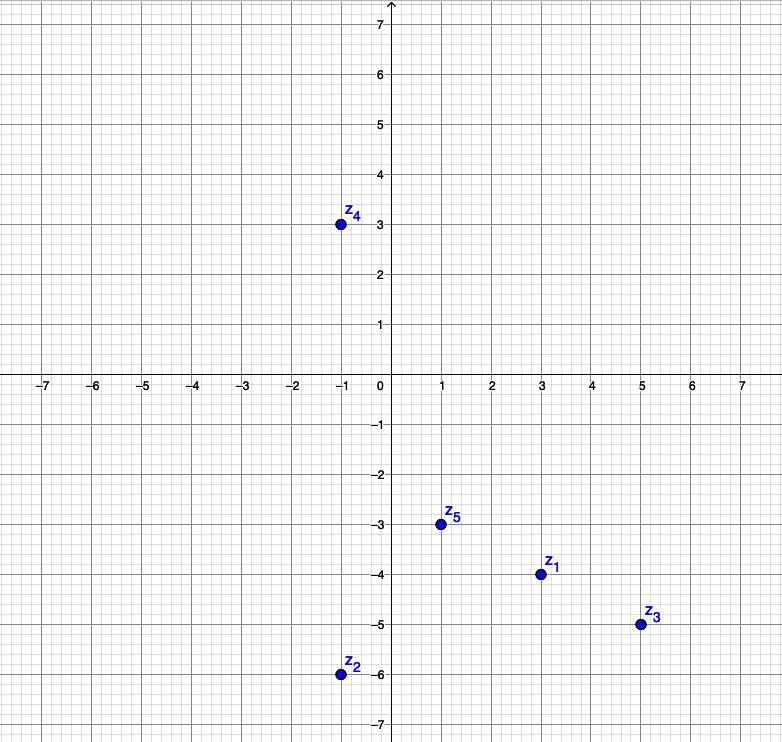
\includegraphics[width=7cm]{Imagenes/1.png}
                \label{fig:nombre_descriptivo}
            \end{figure}
        \end{multicols}
        \item Encuentre el valor de $x$ y de $y$ en los siguientes casos: 
        \begin{enumerate}
            \item $(3, x) = (3, 5)$ 
            \begin{center}
                Solución:
            \end{center}
            \begin{align*}
                x &= 5
            \end{align*}
            \item $(x + 3, 2y) = (y, 2 + x)$
            \begin{center}
                Solución:
            \end{center}
            \begin{align*}
                x + 3 &= y &x + 3 &= -1 \\
                2y &= 2 + x &x &= \boxed{-4} \\
                2y - x &= 2 \\
                2y - (y - 3) &= 2 \\
                2y - y + 3 &= 2 \\
                y + 3 &= 2 \\
                y &= \boxed{-1} 
            \end{align*}
            \item $(x^2-5x+6, 6) = (0,6)$
            \begin{center}
                Solución:
            \end{center}
            \begin{align*}
                x^{2}-5x+6 &= 0 \\
                (x-2)(x-3) &= 0 \\
                x &= \boxed{2, 3}
            \end{align*}
            \item $\dfrac{1}{2}x+\dfrac{2}{3}yi=1-2i$
            \begin{center}
                Solución:
            \end{center}
            \begin{align*}
                \dfrac{1}{2}x+\dfrac{2}{3}yi &= 1-2i &\dfrac{2}{3}yi &= -2i \\
                \dfrac{1}{2}x &= 1 &\dfrac{2}{3}y &= -2 \\
                x &= \boxed{-3} &y &= \boxed{-3} \\
            \end{align*}
            \item $\dfrac{3x+7yi}{4} = \dfrac{2x+1+(8y - 12)i}{5}$
            \begin{center}
                Solución:
            \end{center}
            \begin{align*}
                \dfrac{3x+7yi}{4} &= \dfrac{2x+1+(8y - 12)i}{5} \\
                5(3x+7yi) &= 4(2x+1+(8y - 12)i) \\
                15x+35yi &= 8x+4+32yi-48i \\
                15x-8x+35yi - 32yi &= 4-48i \\
                7x+3yi &= 4-48i
            \end{align*}
            Un conjunto de números complejos solo pueden ser iguales si sus partes reales e imaginarias son iguales, por lo tanto:
            \newline
            \begin{align*}
                7x &= 4 &3y &= -48 \\
                x &= \boxed{\dfrac{4}{7}} &y &= \boxed{-16}
            \end{align*}
        \end{enumerate}
        \item Efectúa las siguientes operaciones:
        \begin{enumerate}
            \item $(-6, 5) + (-3, 4) =$
            \begin{center}
                Solución:
            \end{center}
            \begin{align*}
                (-6, 5) + (-3, 4) &= (-6-3, 5+4) \\
                &= \boxed{(-9, 9)}
            \end{align*}
            \item $(-1, 3) - (5, 7)$
            \begin{center}
                Solución:   
            \end{center}
            \begin{align*}
                (-1, 3) - (5, 7) &= (-1-5, 3-7) \\
                &= \boxed{(-6, -4)}
            \end{align*}
            \item $(-4, -5) + (-3, -9)$
            \begin{center}
                Solución:
            \end{center}
            \begin{align*}
                (-4, -5) + (-3, -9) &= (-4-3, -5-9) \\
                &= \boxed{(-7, -14)}
            \end{align*}
            \item $(-4, -5) - (-12, 1)$
            \begin{center}
                Solución:
            \end{center}
            \begin{align*}
                (-4, -5) - (-12, 1) &= (-4+12, -5-1) \\
                &= \boxed{(8, -6)}
            \end{align*}
            \item $(-7, -8) + (-5, 6) - (-2, -1)$
            \begin{center}
                Solución:
            \end{center}
            \begin{align*}
                (-7, -8) + (-5, 6) - (-2, -1) &= (-7-5+2, -8+6+1) \\
                &= \boxed{(-10, -1)}
            \end{align*}
            \item $(5, -3) - (7, -1) + (10, 8)$
            \begin{center}
                Solución:
            \end{center}
            \begin{align*}
                (5, -3) - (7, -1) + (10, 8) &= (5-7+10, -3+1+8) \\
                &= \boxed{(8, 6)}
            \end{align*}
            \item $(7, -3) \cdotp (-2, 5)$
            \begin{center}
                Solución:
            \end{center}
            \begin{align*}
                (7, -3) \cdotp (-2, 5) &= (7 \cdotp -2 - (-3) \cdotp 5, 7 \cdotp 5 + (-3) \cdotp -2) \\
                &= \boxed{(-4, 29)}
            \end{align*}
            \item $(-9, -5) \cdotp (-8, -9)$
            \begin{center}
                Solución:
            \end{center}
            \begin{align*}
                (-9, -5) \cdotp (-8, -9) &= (-9 \cdotp -8 - (-5) \cdotp -9, -9 \cdotp -9 + (-5) \cdotp -8) \\
                &= \boxed{(47, -81)}
            \end{align*}
            \item $(12, -5) \cdotp (12, -5) - (13, 3) \cdotp (13, -8)$
            \begin{center}
                Solución:
            \end{center}
            \begin{align*}
                (12, -5) \cdotp (12, -5) - (13, 3) \cdotp (13, -8) &= (12 \cdotp 12 - (-5) \cdotp (-5) - (13 \cdotp 13 - 3 \cdotp (-8)) \\
                &= \boxed{(169, 169)}
            \end{align*}
            \item $(3, -8) : (2, -3)$
            \begin{center}
                Solución:
            \end{center}
            \begin{align*}
                (3, -8) : (2, -3) &= \dfrac{(3, -8)}{(2, -3)} \\
                &= \dfrac{(3, -8) \cdotp (2, 3)}{(2, -3) \cdotp (2, 3)} \\
                &= \dfrac{(3 \cdotp 2 - (-8) \cdotp 3, 3 \cdotp 3 + (-8) \cdotp 2)}{(2 \cdotp 2 - (-3) \cdotp 3)} \\
                &= \dfrac{(30, -1)}{(13, 13)} \\
                &= \boxed{\left(\dfrac{30}{13}, \dfrac{-1}{13}\right)}
            \end{align*}
        \end{enumerate}
    \end{enumerate}


\end{document}